%version du vendredi 20 mars 2009 13h21
\chapter{Lecteurs-rédacteurs}

\startchapter







\lettrine[lines=4]{L}{es} situations de type lecteurs-rédacteurs correspondent à l'accès concurrent à une ressource qui est accédée en lecture par certaines tâches, et en écriture par d'autres. Un exemple typique est l'accès à un fichier, qui peut être ouvert simultanément en lecture par plusieurs tâches, mais en écriture par une seule.

\section{Enoncé du problème}
Un ensemble de threads se partagent des données. Les threads de type \emph{lecteur} ne font que consulter les données, tandis que les threads de type \emph{rédacteur} peuvent également les modifier. Les lecteurs effectuent donc des opérations de lecture, et les rédacteurs des opérations d'écriture.

Les opérations de lecture peuvent être concurrentes. En effet, à titre d'exemple, plusieurs thread peuvent accéder à un même fichier en lecture sans risque de trouver le fichier dans un état incohérent. Les écritures sont, par contre, critiques. Si deux threads modifient l'état d'un fichier au même instant, les données contenues dans le fichier risquent fort d'être corrompues. Et de même, si un thread modifie un fichier alors qu'un autre l'accède en lecture, ce dernier a de bonnes chances de se retrouver avec des données incohérentes. Les accès en écriture doivent donc être effectués en exclusion mutuelle: une écriture ne peut être réalisée si une autre écriture est en cours, une lecture ne peut être faite tant qu'une écriture est en cours, et une écriture ne peut débuter que si aucune lecture n'est en cours.

Pour résumer, les tâches se répartissent en 2 sous-ensembles:

\begin{itemize}
\item les lecteurs qui ne peuvent que lire les données, et
\item les rédacteurs qui peuvent modifier les données.
\end{itemize}

Les contraintes du problème sont les suivantes:

\begin{enumerate}
\item plusieurs lecteurs peuvent lire simultanément les données;
\item les rédacteurs s'excluent mutuellement;
\item les lecteurs et les rédacteurs s'excluent mutuellement.
\end{enumerate}

Ce problème des lecteurs-rédacteurs est plus général qu'un simple problème d'exclusion mutuelle, de par ces contraintes.
Il pourrait être résolu grâce au concept de section critique protégeant tous les accès à la ressource lue et écrite. Toutefois, une telle solution empêcherait les lectures concurrentes, ce qui serait dommageable pour les performances du système.

La solution au problème des lecteurs-rédacteurs n'est pas unique. Plusieurs solutions peuvent en effet être proposées, en fonction des priorités choisies:

\begin{enumerate}
\item Priorité aux lecteurs (famine possible des rédacteurs)
\item Priorité aux lecteurs si un lecteur a déjà accès à la ressource (famine possible des lecteurs)
\item  Priorité aux rédacteurs (famine possible des lecteurs)
\item Accès aux données selon les ordres des arrivées. Toutes les demandes des lecteurs qui se suivent sont satisfaites en même temps.
\end{enumerate}

Les sections suivantes présentes quelques solutions, basées sur les sémaphores.

\section{Priorité aux lecteurs}

Un algorithme basé sur la priorité aux lecteurs doit résoudre l'accès à la ressource, en respectant les règles suivantes:
\begin{itemize}
\item Un lecteur peut accéder à la ressource si:
\begin{itemize}
\item le nombre de rédacteurs en cours d'écriture vaut 0
\end{itemize}
\item Un rédacteur peut accéder à la ressource si:
\begin{itemize}
\item le nombre de rédacteurs en cours d'écriture vaut 0
\item ET le nombre de lecteurs en cours de lecture vaut 0
\item ET le nombre de lecteurs en attente de la ressource vaut 0
\end{itemize}
\end{itemize}

Pour ce faire, nous aurons besoin d'une variable comptant le nombre de lectures en cours: \ccode{nbLecteurs}. Pour garantir l'accès concurrent correct, nous devons également exploiter trois sémaphores. Notons que les algorithmes proposés dans ce chapitre font l'hypothèse que la liste d'attente des sémaphores est gérée selon un ordre \textit{FIFO}. Les sémaphores nécessaires sont donc les suivant:

\begin{itemize}
\item \ccode{mutexLecteurs}, qui est en charge de protéger l'accès à la variable \ccode{nbLecteurs}.
\item \ccode{redacteur}, qui permet au premier lecteur qui accède la ressource de bloquer les futurs rédacteurs. Il permet également au rédacteur accédant la ressource de bloquer les lecteurs pendant l'écriture.
\item \ccode{mutexRedacteurs}, qui permet au rédacteur accédant la ressource de bloquer les autres rédacteurs. De ce fait, un seul rédacteur ne peut être en attente du sémaphore \ccode{redacteur}, empêchant ainsi un rédacteur de brûler la priorité à un lecteur.
\end{itemize}

L'algorithme \ref{lectred:prioritelecteur} présente une solution basée sur ces sémaphores, avec priorité aux lecteurs.


\begin{algorithm}[h!tp]
\caption{Lecteurs-rédacteurs: priorité aux lecteurs}\label{lectred:prioritelecteur}
\centering
\begin{tabular}{l}
\lstset{language=C++}
\begin{lstlisting}
typedef struct {
  sem_t mutexLecteurs;
  sem_t mutexRedacteurs;
  sem_t redacteur;
  int nbLecteurs;
} RessourceLectRed;

void initialiseRessource(RessourceLectRed *res) {
  sem_init(&res->mutexLecteurs,0,1);
  sem_init(&res->mutexRedacteurs,0,1);
  sem_init(&res->redacteur,0,1);
  res->nbLecteurs = 0;
}

void debutLecture(RessourceLectRed *res) {
  sem_wait(&res->mutexLecteurs);
  res->nbLecteurs++;
  if (res->nbLecteurs == 1)
    sem_wait(&res->redacteur);
  sem_post(&res->mutexLecteurs);
}

void finLecture(RessourceLectRed *res) {
  sem_wait(&res->mutexLecteurs);
  res->nbLecteurs--;
  if (res->nbLecteurs == 0)
    sem_post(&res->redacteur);
  sem_post(&res->mutexLecteurs);
}

void debutEcriture(RessourceLectRed *res) {
  sem_wait(&res->mutexRedacteurs);
  sem_wait(&res->redacteur);
}

void finEcriture(RessourceLectRed *res) {
  sem_post(&res->redacteur);
  sem_post(&res->mutexRedacteurs);
}
\end{lstlisting}
\end{tabular}

\end{algorithm}

Les fonctions \ccode{debutLecture()} et \ccode{finLecture()} sont appelées par les lecteurs, alors que \ccode{debutEcriture()} et \ccode{finEcriture()} sont appelées par les rédacteurs. Nous utilisons une structure, \ccode{RessourceLectRed}, pour stocker l'ensemble des informations nécessaires à l'accès d'une ressource. De ce fait, les mêmes fonctions peuvent être utilisées pour l'accès à différentes ressources.

Les figures de \ref{fig:lectred1} à \ref{fig:lectred4} montrent l'évolution de l'état des sémaphores au cours du temps. Les trois sémaphores y sont représentés, avec leur liste de threads en attente. Le nuage gauche représente l'ensemble des threads accédant la ressource en un instant précis. Les lecteurs sont représentés par un \emph{L}, les rédacteur l'étant par un \emph{R}. Le numéro suivant la lettre correspond au temps logique auquel le thread a demandé l'accès à la ressource. Les threads sont ainsi numérotés en fonction de l'ordre de leur arrivée, c'est-à-dire, l'ordre dans lequel ils ont appelé \ccode{debutLecture()} ou \ccode{debutEcriture()}.

A la figure \ref{fig:lectred1}, un rédacteur a l'accès à la ressource critique. Il est donc seul à être dans ce cas. Le sémaphore \ccode{redacteur} bloque un seul lecteur. En effet, les rédacteurs successifs sont bloqués par \ccode{mutexRedacteurs}, celui-ci étant réquisitionné par le rédacteur $R1$. Du côté des lecteurs, seul le premier arrivé est bloqué sur le sémaphore \ccode{redacteur}, les autres étant bloqué sur le sémaphore \ccode{mutexLecteurs}, réquisitionné par le premier lecteur.

\begin{figure}[!ht]
  \centering
    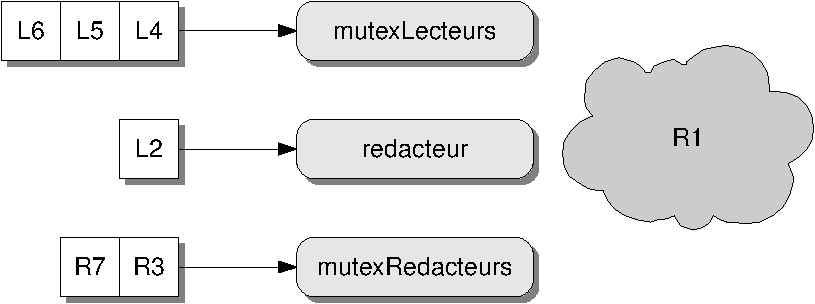
\includegraphics[scale=.7]{lectred1}
    \caption{\label{fig:lectred1}Exemple d'exécution avec priorité aux lecteurs (1)}

\end{figure}

Lorsque le rédacteur $R1$ libère la ressource, il libère le sémaphore \ccode{redacteur} ce qui permet au premier lecteur d'accéder à la ressource.
Il libère ensuite le sémaphore \ccode{mutexRedacteurs}. Le rédacteur $R3$ se place donc en attente sur le sémaphore \ccode{redacteur}, après le lecteur $L2$.
Le lecteur $L2$ relâche donc le sémaphore \ccode{mutexLecteurs}, ce qui permet à tous les lecteurs en attente d'accéder à la ressource, et le système se retrouve dans l'état illustré par la figure \ref{fig:lectred2}.

\begin{figure}[!ht]
  \centering
    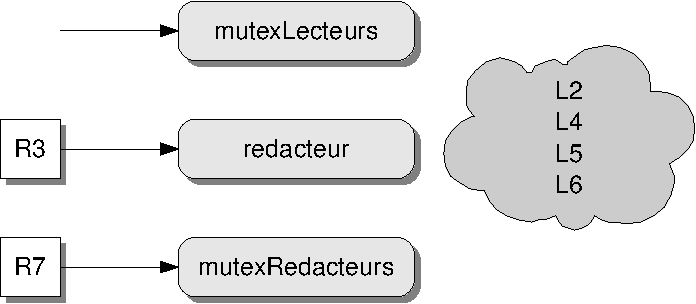
\includegraphics[scale=.7]{lectred2}
    \caption{\label{fig:lectred2}Exemple d'exécution avec priorité aux lecteurs (2)}

\end{figure}

Lorsque de nouveaux rédacteurs désirent accéder à la ressource, ils sont bloqués par le sémaphore \ccode{mutexRedacteurs}. Les lecteurs désirant effectuer la même action sont par contre autorisés à accéder à la ressource. La figure \ref{fig:lectred3} montre l'état du système après l'arrivée de deux rédacteurs et d'un lecteur. $L9$ se retrouve en accès de ressource, alors que $R8$ et $R10$ sont bloqués.

\begin{figure}[!ht]
  \centering
    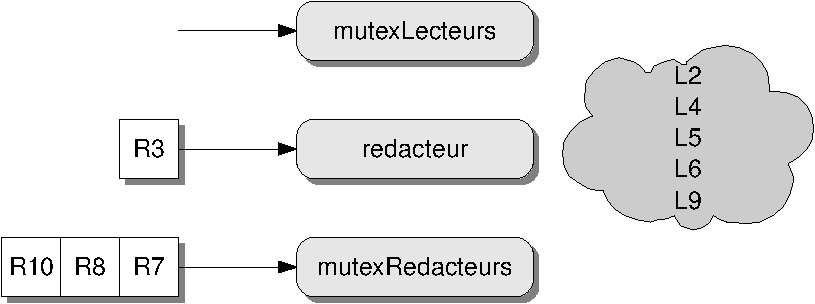
\includegraphics[scale=.7]{lectred3}
    \caption{\label{fig:lectred3}Exemple d'exécution avec priorité aux lecteurs (3)}

\end{figure}

Lorsque tous les lecteurs ont relâché la ressource, le rédacteur $R3$, qui était bloqué par le sémaphore \ccode{redacteur} peut enfin y avoir accès.
La figure \ref{fig:lectred4} illustre cette situation.
Remarquez que la file d'attente associée à \ccode{redacteur} reste vide car $R3$ bloque toujours les rédacteurs par son sémaphore \ccode{mutexRedacteurs}. Un nouvel lecteur qui se présenterait pourra alors se placer à la tête de cette file et ainsi dépasser tous les rédacteurs présents pour prendre la ressource aussitôt que $R3$ libère \ccode{redacteur}.

\begin{figure}[!ht]
  \centering
    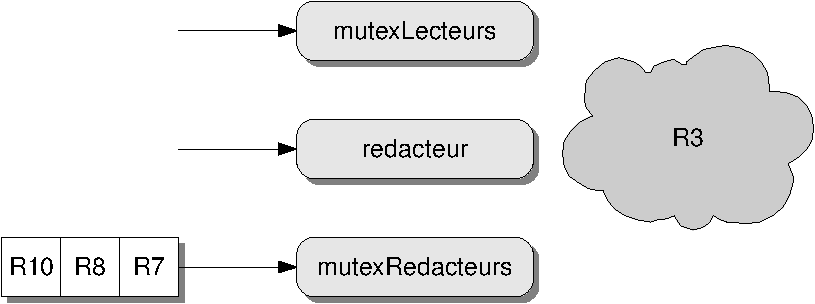
\includegraphics[scale=.7]{lectred4}
    \caption{\label{fig:lectred4}Exemple d'exécution avec priorité aux lecteurs (4)}

\end{figure}

Nous pouvons noter que cet algorithme permet aux lecteurs de se coaliser pour empêcher l'accès aux rédacteurs. En effet, si un nouveau lecteur accède à la ressource avant que tous les lecteurs ne l'aient relâchée, alors les rédacteurs n'auront jamais accès à la ressource.

Le programme \ref{lectredtest} permet de lancer concurremment des lectures et écritures, et peut être exploité pour l'ensemble des exemples de ce chapitre. Il crée des threads rédacteurs et lecteurs et les laisse tenter d'accéder à une ressource hypothétique. Il est à noter que ce programme ne vérifie pas que l'algorithme est correct. Un exercice en fin de chapitre propose d'y ajouter la vérification.

\begin{algorithm}[h!tp]
\caption{Lecteurs-rédacteurs: Programme de test}\label{lectredtest}
\centering
\begin{tabular}{l}
\lstset{language=C++}
\begin{lstlisting}
#define NUM_THREADS_REDACTEUR   1
#define NUM_THREADS_LECTEUR     3

static RessourceLectRed ressource;

void *tacheRedacteur(void *arg) {
  int tid = (int)arg;
  while (true) {
    debutEcriture(&ressource);
    printf("Tache %d: écriture\n",tid);
    finEcriture(&ressource);
  }
  pthread_exit(NULL);
}

void *tacheLecteur(void *arg) {
  int tid  = (int)arg;
  while (true) {
    debutLecture(&ressource);
    printf("Tache %d: lecture\n",tid);
    finLecture(&ressource);
  }
  pthread_exit(NULL);
}

int main(int argc, char *argv[]) {
  pthread_t threadsRed[NUM_THREADS_REDACTEUR];
  pthread_t threadsLec[NUM_THREADS_LECTEUR];
  int t;
  initialiseRessource(&ressource);
  for (t = 0; t < NUM_THREADS_LECTEUR; t++) {
    printf("Création du lecteur %d\n",t);
    if (pthread_create(&threadsLec[t], NULL, tacheLecteur, (void *)t) == 0)
      exit(-1);
  }
  for (t = 0; t < NUM_THREADS_REDACTEUR; t++) {
    printf("Création du rédacteur %d\n",t);
    if (pthread_create(&threadsRed[t], NULL, tacheRedacteur, (void *)t) == 0)
      exit(-1);
  }
  for (t = 0; t < NUM_THREADS_LECTEUR; t++)
    pthread_join(threadsLec[t],NULL);
  for (t = 0; t < NUM_THREADS_REDACTEUR; t++)
    pthread_join(threadsRed[t],NULL);
  return 0;
}
\end{lstlisting}
\end{tabular}

\end{algorithm}

Nous pouvons également noter que ce programme de test, ainsi la manière dont sont réalisés les différents protocoles présentés dans ce chapitre, peuvent être considérés comme légèrement risqués. En effet, la variable de type \ccode{RessourceLectRed} est déclarée dans le programme principal. En théorie, seules les fonctions de début et de fin de lecture et d'écriture y font référence. Pour que le fonctionnement soit correct, il faudrait garantir que le programme principal n'agisse pas directement sur cette structure, sans quoi le système risquerait de se retrouver dans un état incohérent. Ceci pourrait aisément être réalisé grâce à une meilleure encapsulation, mais la compréhension du chapitre ne nécessitant pas de telles contraintes, l'exercice est laissé au bon vouloir du lecteur.

L'algorithme \ref{lectred:prioritelecteur} peut être légèrement modifié pour donner priorité aux lecteurs uniquement si une lecture est en cours.
Ce nouvel algorithme \ref{lectred:prioritelecteurcourant} permet toujours aux lecteurs de se coaliser, comme précédemment. Si plusieurs rédacteurs veulent accéder à la ressource pendant qu'elle est occupée par des lecteurs, le premier rédacteur accèdera dès que les lecteurs seront tous sortis, mais les rédacteurs en attente auront accès avant les lecteurs futurs. En effet, le prochain lecteur qui se présentera se placera derrière ces rédacteurs et tous ceux qui ont fait une demande avant le lecteur.

\begin{algorithm}[h!tp]
\caption{Lecteurs-rédacteurs: priorité aux lecteurs uniquement si une lecture est en cours}\label{lectred:prioritelecteurcourant}
\centering
\begin{tabular}{l}
\lstset{language=C++}
\begin{lstlisting}
typedef struct {
  sem_t mutexLecteurs;
  sem_t redacteur;
  int nbLecteurs;
} RessourceLectRed;

void initialiseRessource(RessourceLectRed *res) {
  sem_init(&res->mutexLecteurs,0,1);
  sem_init(&res->redacteur,0,1);
  res->nbLecteurs = 0;
}

void debutLecture(RessourceLectRed *res) {
  sem_wait(&res->mutexLecteurs);
  res->nbLecteurs++;
  if (res->nbLecteurs == 1)
    sem_wait(&res->redacteur);
  sem_post(&res->mutexLecteurs);
}

void finLecture(RessourceLectRed *res) {
  sem_wait(&res->mutexLecteurs);
  res->nbLecteurs--;
  if (res->nbLecteurs == 0)
    sem_post(&res->redacteur);
  sem_post(&res->mutexLecteurs);
}

void debutEcriture(RessourceLectRed *res) {
  sem_wait(&res->redacteur);
}

void finEcriture(RessourceLectRed *res) {
  sem_post(&res->redacteur);
}
\end{lstlisting}
\end{tabular}

\end{algorithm}

Il également possible d'implémenter l'algorithme \ref{lectred:prioritelecteur} d'une autre manière. Il s'agit d'un modèle permettant de dériver plusieurs solutions, en fonction des priorités à accorder. Ce modèle de solution se prête également à la résolution de problèmes s'apparentant aux lecteurs-rédacteurs, tels que le passage d'un pont, les giratoires, ou les ressources multiples. Pour ce modèle, nous utilisons les informations contenues dans la structure suivante:

\begin{lstlisting}
typedef struct {
  sem_t mutex;
  sem_t lecteurs;
  sem_t redacteur;
  int nbLecteurs;
  int lectEnAttente;
  int redEnAttente;
  bool unRedacteur;
} RessourceLectRed;
\end{lstlisting}

\begin{itemize}
\item \ccode{mutex} protège l'accès aux variables partagées, tous les threads risquant d'en effectuer des accès concurrents;
\item \ccode{lecteurs} est un sémaphore permettant de bloquer les lecteurs;
\item \ccode{redacteurs} est un sémaphore permettant de bloquer les rédacteurs;
\item \ccode{nbLecteurs} sert à compter le nombre de lecteurs en phase de lecture;
\item \ccode{lectEnAttente} sert à compter le nombre de lecteurs en attente de la ressource;
\item \ccode{redEnAttente} sert à compter le nombre de rédacteurs en attente de la ressource;
\item \ccode{unRedacteur} indique si un rédacteur est en phase d'écriture. Il s'agit d'un booléen, étant donné qu'un seul rédacteur ne peut être en écriture à un instant donné. Cette variable pourrait être un entier dans le cas d'un problème différent de celui du simple lecteurs-rédacteurs.
\end{itemize}

L'algorithme \ref{lectred:prioritelecteurgenerale} présente la solution basée sur ce modèle.

\begin{algorithm}[h!tp]
\caption{Lecteurs-rédacteurs: priorité aux lecteurs, solution générale}\label{lectred:prioritelecteurgenerale}
\centering
\begin{tabular}{l}
\lstset{language=C++}
\begin{lstlisting}
void initialiseRessource(RessourceLectRed *res) {
  sem_init(&res->mutex,0,1);
  sem_init(&res->lecteurs,0,0);
  sem_init(&res->redacteur,0,0);
  res->nbLecteurs = 0;
  res->lectEnAttente = 0;
  res->redEnAttente = 0;
  res->unRedacteur = false;
}

void debutLecture(RessourceLectRed *res) {
  sem_wait(&res->mutex);
  if (res->unRedacteur) {
    res->lectEnAttente++;
    sem_post(&res->mutex);
    sem_wait(&res->lecteurs);
  }
  else {
    res->nbLecteurs++;
    sem_post(&res->mutex);
  }
}

void finLecture(RessourceLectRed *res) {
  sem_wait(&res->mutex);
  res->nbLecteurs--;
  if (res->nbLecteurs == 0 && res->redEnAttente > 0) {
    res->unRedacteur = true;
    res->redEnAttente--;
    sem_post(&res->redacteur);
  }
  sem_post(&res->mutex);
}

void debutEcriture(RessourceLectRed *res) {
  sem_wait(&res->mutex);
  if (res->unRedacteur || res->nbLecteurs + res->lectEnAttente > 0) {
    res->redEnAttente++;
    sem_post(&res->mutex);
    sem_wait(&res->redacteur);
  }
  else {
    res->unRedacteur = true;
    sem_post(&res->mutex);
  }
}

void finEcriture(RessourceLectRed *res) {
  int i;
  sem_wait(&res->mutex);
  res->unRedacteur = false;
  if (res->lectEnAttente > 0) {
    for (i = 0; i < res->lectEnAttente; i++)
      sem_post(&res->lecteurs);
    res->nbLecteurs = res->lectEnAttente;
    res->lectEnAttente = 0;
  }
  else if (res->redEnAttente > 0) {
    res->unRedacteur = true;
    res->redEnAttente--;
    sem_post(&res->redacteur);
  }
  sem_post(&res->mutex);
}
\end{lstlisting}
\end{tabular}

\end{algorithm}


\section{Priorité égale}
Un algorithme basé sur une priorité égale doit résoudre l'accès à la ressource, en respectant les règles suivantes:
\begin{itemize}
\item Un lecteur peut accéder à la ressource uniquement si le nombre de rédacteurs en cours d'écriture vaut 0
\item Un rédacteur peut accéder à la ressource si:
\begin{itemize}
\item le nombre de rédacteurs en cours d'écriture vaut 0
\item ET le nombre de lecteurs en cours de lecture est également 0
\end{itemize}
\end{itemize}

Pour ce faire, nous aurons besoin d'une variable comptant le nombre de lectures en cours: \ccode{nbLecteurs}. Pour garantir l'accès concurrent correct, nous devons également exploiter trois sémaphores.

Les sémaphores nécessaires sont les suivants:
\begin{itemize}
\item \ccode{mutex}, qui est en charge de protéger l'accès à la variable \ccode{nbLecteurs}.
\item \ccode{redacteur}, qui permet au premier lecteur qui accède la ressource de bloquer les futurs rédacteurs. Il permet également au rédacteur accédant la ressource de bloquer les lecteurs pendant l'écriture.
\item \ccode{fifo}, une file d'attente dans laquelle passent tous les lecteurs et rédacteurs.
\end{itemize}

L'algorithme \ref{lectred:prioriteegale} présente une solution avec priorité égale, basée sur ces trois sémaphores.

\begin{algorithm}[h!tp]
\caption{Lecteurs-rédacteurs: priorité égale}\label{lectred:prioriteegale}
\centering
\begin{tabular}{l}
\lstset{language=C++}
\begin{lstlisting}
typedef struct {
  sem_t mutex;
  sem_t fifo;
  sem_t redacteur;
  int nbLecteurs;
} RessourceLectRed;

void initialiseRessource(RessourceLectRed *res) {
  sem_init(&res->mutex,0,1);
  sem_init(&res->fifo,0,1);
  sem_init(&res->redacteur,0,1);
  res->nbLecteurs = 0;
}

void debutLecture(RessourceLectRed *res) {
  sem_wait(&res->fifo);
  sem_wait(&res->mutex);
  res->nbLecteurs++;
  if (res->nbLecteurs == 1)
    sem_wait(&res->redacteur);
  sem_post(&res->mutex);
  sem_post(&res->fifo);
}

void finLecture(RessourceLectRed *res) {
  sem_wait(&res->mutex);
  res->nbLecteurs--;
  if (res->nbLecteurs == 0)
    sem_post(&res->redacteur);
  sem_post(&res->mutex);
}

void debutEcriture(RessourceLectRed *res) {
  sem_wait(&res->fifo);
  sem_wait(&res->redacteur);
}

void finEcriture(RessourceLectRed *res) {
  sem_post(&res->redacteur);
  sem_post(&res->fifo);
}
\end{lstlisting}
\end{tabular}

\end{algorithm}

Le sémaphore \ccode{fifo} est le point central de l'algorithme. Il sert à préserver l'ordre des demandes et il est initialisé à 1, permettant au premier thread arrivé de passer directement. Un seul thread peut donc posséder ce sémaphore à un instant donné, ce qui correspond à un simple verrou. Un seul thread étant en possession du verrou, nous pouvons observer que les rédacteurs acquièrent le verrou dans \ccode{debutEcriture()}, et le relâchent dans \ccode{finEcriture()}. De ce fait, un seul rédacteur ne peut être actif à un instant donné. Du côté des lecteurs, ce même verrou n'est réquisitionné que dans \ccode{debutLecture()}, afin d'autoriser le premier lecteur disponible à accéder la ressource. Le premier à passer va alors bloquer les rédacteurs, grâce au verrou \ccode{redacteur}.

Il est intéressant de noter que les interblocage sont évités grâce
à l'ordre des appels des sémaphores \ccode{fifo} et \ccode{redacteur} qui est effectué pour les lecteurs et les rédacteurs.
Si tel n'avait pas été le cas, le système aurait risqué un interblocage.

\section{Priorité aux rédacteurs}
Un algorithme basé sur une priorité aux rédacteurs doit résoudre l'accès à la ressource, en respectant les règles suivantes:
\begin{itemize}
\item Un lecteur peut accéder à la ressource si:
\begin{itemize}
\item le nombre de rédacteurs en cours d'écriture vaut 0
\item ET le nombre de rédacteurs en attente d'écriture vaut également 0
\end{itemize}
\item Un rédacteur peut accéder à la ressource si:
\begin{itemize}
\item le nombre de rédacteurs en cours d'écriture vaut 0
\item ET le nombre de lecteurs en cours de lecture vaut également 0
\end{itemize}
\end{itemize}

Dans ce cas, à l'instar des lecteurs dans le cas d'une priorité les avantageant, les rédacteurs pourront se coaliser pour empêcher les lecteurs d'accéder à la ressource.

Pour cet algorithme, nous aurons besoin d'une variable comptant le nombre de lectures en cours, \ccode{nbLecteurs}, ainsi qu'une comptant le nombre de rédacteurs en attente d'écriture ou en cours d'écriture. Pour garantir l'accès concurrent correct, nous devons également exploiter cinq sémaphores.

Les sémaphores nécessaires sont donc les suivants:
\begin{itemize}
\item \ccode{mutexLecteurs}, qui permet de bloquer les lecteurs pendant que des écritures sont en cours.
\item \ccode{mutexRedacteurs}, qui permet de bloquer les rédacteurs pendant que des écritures ou des lectures sont en cours.
\item \ccode{redacteur}, qui permet au premier lecteur qui accède la ressource de bloquer les potentiels rédacteurs.
\item \ccode{lecteur}, qui permet au premier rédacteur arrivé de bloquer les potentiels futurs lecteurs.
\item \ccode{mutex}, qui est en charge de protéger l'accès à la variable \ccode{nbLecteurs}.
\end{itemize}

L'algorithme \ref{lectred:prioriteredacteurs} présente une solution avec priorité aux rédacteurs, basée sur ces cinq sémaphores.


\begin{algorithm}[h!tp]
\caption{Lecteurs-rédacteurs: priorité aux rédacteurs}\label{lectred:prioriteredacteurs}
\centering
\begin{tabular}{l}
\lstset{language=C++}
\begin{lstlisting}
typedef struct {
  sem_t mutexLecteurs;
  sem_t mutexRedacteurs;
  sem_t lecteur;
  sem_t redacteur;
  sem_t mutex;
  int nbLecteurs;
  int nbRedacteurs;
} RessourceLectRed;

void initialiseRessource(RessourceLectRed *res) {
  sem_init(&res->mutexLecteurs,0,1);
  sem_init(&res->mutexRedacteurs,0,1);
  sem_init(&res->redacteur,0,1);
  sem_init(&res->lecteur,0,1);
  sem_init(&res->mutex,0,1);
  res->nbLecteurs = 0;
  res->nbRedacteurs = 0;
}

void debutLecture(RessourceLectRed *res) {
  sem_wait(&res->mutexLecteurs);
  sem_wait(&res->lecteur);
  sem_wait(&res->mutex);
  res->nbLecteurs++;
  if (res->nbLecteurs == 1)
    sem_wait(&res->redacteur);
  sem_post(&res->mutex);
  sem_post(&res->lecteur);
  sem_post(&res->mutexLecteurs);
}

void finLecture(RessourceLectRed *res) {
  sem_wait(&res->mutex);
  res->nbLecteurs--;
  if (res->nbLecteurs == 0)
    sem_post(&res->redacteur);
  sem_post(&res->mutex);
}

void debutEcriture(RessourceLectRed *res) {
  sem_wait(&res->mutexRedacteurs);
  res->nbRedacteurs++;
  if (res->nbRedacteurs == 1)
    sem_wait(&res->lecteur);
  sem_post(&res->mutexRedacteurs);
  sem_wait(&res->redacteur);
}

void finEcriture(RessourceLectRed *res) {
  sem_post(&res->redacteur);
  sem_wait(&res->mutexRedacteurs);
  res->nbRedacteurs--;
  if (res->nbRedacteurs == 0)
    sem_post(&res->lecteur);
  sem_post(&res->mutexRedacteurs);
}
\end{lstlisting}
\end{tabular}

\end{algorithm}

Nous pouvons noter une certaine symétrie entre les lecteurs et les rédacteurs, chacuns étant capables de bloquer les autres. Le premier lecteur à accéder à la ressource bloque les rédacteurs, grâce au sémaphore \ccode{redacteur}. En fin de lecture, le dernier lecteur à relâcher la ressource va alors débloquer les rédacteurs. De manière symétrique, le premier rédacteur à accéder à la ressource va bloquer l'ensemble des lecteurs grâce au sémaphore \ccode{lecteur}, et le dernier rédacteur à relâcher la ressource va débloquer les lecteurs.

\section{Conclusion}

Le problème des lecteurs-rédacteurs peut être résolu de différentes manières, tel que démontré par les deux algorithmes pour la priorité aux lecteurs. Ce paradigme peut également servir à modéliser différents types de systèmes tels que l'accès à un pont à voie unique par des voitures venant des deux sens, par exemple. De tels problèmes seront abordés en exercices.


\section{Exercices}

\startexercice

Dans l'algorithme \ref{lectred:prioritelecteur}, pourrions-nous remplacer les sémaphores par des verrous? Montrer comment.

\startexercice

Reprendre l'algorithme général avec priorité aux lecteurs (algorithme \ref{lectred:prioritelecteurgenerale}), et l'adapter pour proposer une nouvelle solution qui donne priorité aux rédacteurs.

\startexercice

Mettre au point un programme capable de tester un des algorithmes présentés dans ce chapitre.

\startexercice

Une application est composée de threads de deux classes, A et B. Une ressource est partagée entre tous les threads, selon les contraintes suivantes:
\begin{enumerate}
\item Les threads de classe A peuvent accéder concurremment  à la ressource.
\item Les threads de classe B peuvent accéder concurremment à la ressource.
\item Les threads de différente classe ne peuvent accéder à la ressource au même instant. Autrement dit, les threads de différente classe s'excluent mutuellement.
\end{enumerate}

Proposer un algorithme permettant de gérer l'accès à la ressource, en s'inspirant des solutions du chapitre. Considérer une solution où la coalition est possible entre threads d'une même classe.

%\subsection*{Exercice 6}
%En reprenant l'algorithme précédent, proposer une solution où la coalition n'est pas tolérée. La séquence d'accès doit donc y être respectée.
%CEZ: Je ne comprend pas: c'est l'algo égalitaire!

\startexercice

Proposer un scénario semblable aux figures \ref{fig:lectred1} à \ref{fig:lectred4}, illustrant le fonctionnement de l'algorithme
\ref{lectred:prioritelecteurcourant}, où les lecteurs sont prioritaires que si une lecture est en cours.
